% Created 2021-03-30 Tue 13:12
% Intended LaTeX compiler: pdflatex

  \documentclass[english]{article}
  \usepackage[T1, T2A]{fontenc}
\usepackage[lutf8]{luainputenc}
\usepackage[english, russian]{babel}
\usepackage{minted}
\usepackage{graphicx}
\usepackage{longtable}
\usepackage{hyperref}
\usepackage{xcolor}
\usepackage{natbib}
\usepackage{amssymb}
\usepackage{stmaryrd}
\usepackage{amsmath}
\usepackage{caption}
\usepackage{mathtools}
\usepackage{amsthm}
\usepackage{tikz}
\usepackage{grffile}
\usepackage{extarrows}
\usepackage{wrapfig}
\usepackage{rotating}
\usepackage{placeins}
\usepackage[normalem]{ulem}
\usepackage{amsmath}
\usepackage{textcomp}
\usepackage{capt-of}
  
  \usepackage{geometry}
  \geometry{a4paper,left=2.5cm,top=2cm,right=2.5cm,bottom=2cm,marginparsep=7pt, marginparwidth=.6in}
   \usepackage{hyperref}
 \hypersetup{
     colorlinks=true,
     linkcolor=blue,
     filecolor=orange,
     citecolor=black,      
     urlcolor=cyan,
     }

\usetikzlibrary{decorations.markings}
\usetikzlibrary{cd}
\usetikzlibrary{patterns}
\usetikzlibrary{automata, arrows}

\newcommand\addtag{\refstepcounter{equation}\tag{\theequation}}
\newcommand{\eqrefoffset}[1]{\addtocounter{equation}{-#1}(\arabic{equation}\addtocounter{equation}{#1})}


\newcommand{\R}{\mathbb{R}}
\renewcommand{\C}{\mathbb{C}}
\newcommand{\N}{\mathbb{N}}
\newcommand{\rank}{\text{rank}}
\newcommand{\const}{\text{const}}
\newcommand{\grad}{\text{grad}}

\newcommand{\todo}{{\color{red}\fbox{\text{Доделать}}}}
\newcommand{\fixme}{{\color{red}\fbox{\text{Исправить}}}}

\newcounter{propertycnt}
\setcounter{propertycnt}{1}
\newcommand{\beginproperty}{\setcounter{propertycnt}{1}}

\theoremstyle{plain}
\newtheorem{propertyinner}{Свойство}
\newenvironment{property}{
  \renewcommand\thepropertyinner{\arabic{propertycnt}}
  \propertyinner
}{\endpropertyinner\stepcounter{propertycnt}}
\newtheorem{axiom}{Аксиома}
\newtheorem{lemma}{Лемма}
\newtheorem{manuallemmainner}{Лемма}
\newenvironment{manuallemma}[1]{%
  \renewcommand\themanuallemmainner{#1}%
  \manuallemmainner
}{\endmanuallemmainner}

\theoremstyle{remark}
\newtheorem*{remark}{Примечание}
\newtheorem*{solution}{Решение}
\newtheorem{corollary}{Следствие}[theorem]
\newtheorem*{examp}{Пример}
\newtheorem*{observation}{Наблюдение}

\theoremstyle{definition}
\newtheorem{task}{Задача}
\newtheorem{theorem}{Теорема}[section]
\newtheorem*{definition}{Определение}
\newtheorem*{symb}{Обозначение}
\newtheorem{manualtheoreminner}{Теорема}
\newenvironment{manualtheorem}[1]{%
  \renewcommand\themanualtheoreminner{#1}%
  \manualtheoreminner
}{\endmanualtheoreminner}
\captionsetup{justification=centering,margin=2cm}
\newenvironment{colored}[1]{\color{#1}}{}

\tikzset{->-/.style={decoration={
  markings,
  mark=at position .5 with {\arrow{>}}},postaction={decorate}}}
\makeatletter
\newcommand*{\relrelbarsep}{.386ex}
\newcommand*{\relrelbar}{%
  \mathrel{%
    \mathpalette\@relrelbar\relrelbarsep
  }%
}
\newcommand*{\@relrelbar}[2]{%
  \raise#2\hbox to 0pt{$\m@th#1\relbar$\hss}%
  \lower#2\hbox{$\m@th#1\relbar$}%
}
\providecommand*{\rightrightarrowsfill@}{%
  \arrowfill@\relrelbar\relrelbar\rightrightarrows
}
\providecommand*{\leftleftarrowsfill@}{%
  \arrowfill@\leftleftarrows\relrelbar\relrelbar
}
\providecommand*{\xrightrightarrows}[2][]{%
  \ext@arrow 0359\rightrightarrowsfill@{#1}{#2}%
}
\providecommand*{\xleftleftarrows}[2][]{%
  \ext@arrow 3095\leftleftarrowsfill@{#1}{#2}%
}
\makeatother
\author{Ilya Yaroshevskiy}
\date{\today}
\title{Практика 8}
\hypersetup{
 pdfauthor={Ilya Yaroshevskiy},
 pdftitle={Практика 8},
 pdfkeywords={},
 pdfsubject={},
 pdfcreator={Emacs 28.0.50 (Org mode )}, 
 pdflang={English}}
\begin{document}

\maketitle
\tableofcontents

\begin{task}
\[ f(x) = \begin{cases}
0 & x < 0 \\
ax & 0 \le x \le 2 \\
0 & x > 2
\end{cases}\]
Найти \(a\), мат. ожидание и т.д.
\end{task}
\begin{solution}
\begin{enumerate}
\item Надо проверить условие нормировки. По условию нормирвки:
\[ \int\limits_{-\infty}^\infty f(x) dx = 1 \Rightarrow \int\limits_0^2 ax dx = a\cdot \frac{x^2}{2} \bigg|_0^2 = 2a = 1 \Rightarrow a = \frac{1}{2}  \]
\item \[ E\xi = \int\limits_{- \infty}^\infty x f(x) dx = \int_0^2 x \cdot \frac{x}{2} dx = \frac{1}{2} \cdot \frac{x^3}{3} \bigg|_0^1 = \frac{4}{3} \]
\item \[ D\xi = \int_{ -\infty}^\infty x^2 f(x) dx - (E\xi)^2 = \int_0^2 x^2 \cdot \frac{x}{2} dx  - \left(\frac{4}{3}\right)^2 = \frac{1}{2} \cdot \frac{x^4}{4} \bigg|_0^2 - \frac{16}{9} = 2 - \frac{16}{9} = \frac{2}{9} \]
\item \[ F(x) = \int_{- \infty}^x f(x) dx \]
\begin{itemize}
\item при \(x < 0\) \(F(x) = 0\)
\item при \(0 \le x \le 2\) \(F(x) = \int_0^x \frac{x}{2} dx = \frac{x^2}{4}\bigg|_0^x = \frac{x^2}{4}\)
\item при \(x > 2\) \(F(x) = 0\)
\end{itemize}
\[ F(x) = \begin{cases}
   0 & x < 0 \\
   \frac{x^2}{4} & 0 \le x \le 2 \\
   1 & x > 2
   \end{cases} \]
\item \(p(\alpha < \xi < \beta) = F(\beta) - F(\alpha)\)
\[ p \left(\frac{1}{2} < \xi < \frac{3}{2}\right) = F \left(\frac{3}{2}\right)  - F \left(\frac{1}{2}\right) = F \left(\frac{\left(\frac{3}{2}\right)^2}{4}\right) - F \left(\frac{\left(\frac{1}{2}\right)^2}{4}\right) = \frac{9}{16} - \frac{1}{16} = \frac{1}{2}\]
\item \begin{center}
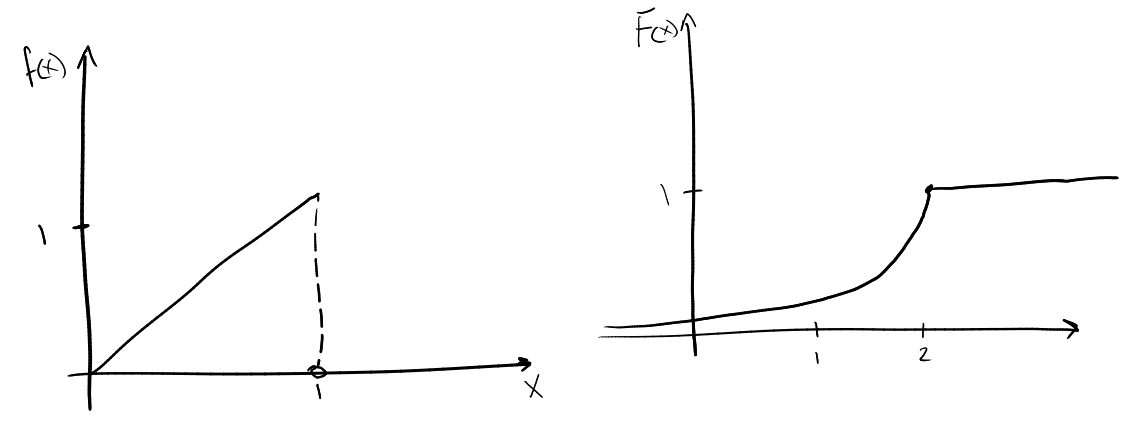
\includegraphics[scale=0.3]{8_1.png}
\end{center}
\end{enumerate}
\end{solution}
\begin{task}
\[ F(x) = \begin{cases}
0 & x < 1 \\
\frac{A}{x^4} + B & x \ge 1
\end{cases}\]
\end{task}
\begin{task}
Условия:
\begin{enumerate}
\item \begin{enumerate}
\item \[ \lim_{x \to \infty} F(x) = 1 \], \(F(x)\) --- непрерывная
\item \[ \lim_{x - 0 \to 1} F(x) = \lim_{x + 0 \to 1} F(x) \]
\end{enumerate}
Отсюда находим константы \(A, B\)
\begin{enumerate}
\item \[ \lim_{x \to \infty} \underbrace{\frac{A}{x^4}}_{\to 0} + B = 1 \Rightarrow B = 1 \]
\item \[ \lim_{X -0 \to 1} 0 = \lim_{x + 0 \to 1} \frac{A}{x^4} + 1 \Rightarrow A = -1 \]
\end{enumerate}
\item \[ f(x) = F'(x) = \begin{cases}
   0 & x < 1 \\
   \frac{4}{x^5} & x \ge 1
   \end{cases} \]
\item \[ E\xi = \int_{-\infty}^\infty  x f(x) dx = \int_1^\infty x \cdot \frac{4}{x^5} dx = 4 \cdot \frac{x^{-3}}{-3} \bigg|_1^\infty = - \frac{4}{3} \lim_{x \to \infty} \left(\frac{1}{x^3} - \frac{1}{1^3}\right) = \frac{4}{3}  \]
\item \[ D\xi = \int_{-\infty}^\infty x^2 fx dx - (E\xi)^2 = \int_1^\infty x^2 \cdot \frac{4}{x^5} dx - \frac{16}{9} = 4\cdot \frac{x^{-2}}{-2} \bigg|_1^\infty - \frac{16}{9} = -2\lim_{x \to \infty} \left(\frac{1}{x^2} - 1\right) - \frac{16}{9} = 2 - \frac{16}{9} = \frac{2}{9} \]
\item \[ \sigma = \frac{\sqrt{2}}{3} \]
\item \[ p(0 < \xi < 2) = F(2) - F(0) = \left(1 - \frac{1}{16}\right) - 0 = \frac{15}{16} \]
\[ p(\xi > 4) = 1 - P(\xi < 4) = 1 - F(4)\todo \]
\end{enumerate}
\end{task}
\section{ДЗ}
\label{sec:orgceadee2}
\begin{task}
\[ F(x) = \begin{cases}
0 & x < -2 \\
Ax + b & -2 \le x \le 2 \\
1 & x > 2
\end{cases}\]
Найти \(A, B\),  плотность \(f(x)\), числовые характеристики, \(p(-1 < \xi < 1)\), графики
\end{task}
\begin{task}
\[ f(x) = \begin{cases}
0 & x < 0 \\
A \sin x & 0 \le x \le \pi \\
0 & x > \pi
\end{cases}\]
Найти \(A\), \(F(x)\), \(p(\frac{\pi}{4} < \xi < \frac{\pi}{2})\), графики
\end{task}
\begin{task}
Двое человек договорились всетретиься между 12:00 и 13:00. Случайная
величина --- вермя ожидания пришедшего первым. Найти матиматическое
ожидание и дисперсию
\end{task}
\end{document}
